% Options for packages loaded elsewhere
\PassOptionsToPackage{unicode}{hyperref}
\PassOptionsToPackage{hyphens}{url}
\PassOptionsToPackage{dvipsnames,svgnames,x11names}{xcolor}
%
\documentclass[
  letterpaper,
  DIV=11,
  numbers=noendperiod]{scrreprt}

\usepackage{amsmath,amssymb}
\usepackage{lmodern}
\usepackage{iftex}
\ifPDFTeX
  \usepackage[T1]{fontenc}
  \usepackage[utf8]{inputenc}
  \usepackage{textcomp} % provide euro and other symbols
\else % if luatex or xetex
  \usepackage{unicode-math}
  \defaultfontfeatures{Scale=MatchLowercase}
  \defaultfontfeatures[\rmfamily]{Ligatures=TeX,Scale=1}
\fi
% Use upquote if available, for straight quotes in verbatim environments
\IfFileExists{upquote.sty}{\usepackage{upquote}}{}
\IfFileExists{microtype.sty}{% use microtype if available
  \usepackage[]{microtype}
  \UseMicrotypeSet[protrusion]{basicmath} % disable protrusion for tt fonts
}{}
\makeatletter
\@ifundefined{KOMAClassName}{% if non-KOMA class
  \IfFileExists{parskip.sty}{%
    \usepackage{parskip}
  }{% else
    \setlength{\parindent}{0pt}
    \setlength{\parskip}{6pt plus 2pt minus 1pt}}
}{% if KOMA class
  \KOMAoptions{parskip=half}}
\makeatother
\usepackage{xcolor}
\setlength{\emergencystretch}{3em} % prevent overfull lines
\setcounter{secnumdepth}{5}
% Make \paragraph and \subparagraph free-standing
\ifx\paragraph\undefined\else
  \let\oldparagraph\paragraph
  \renewcommand{\paragraph}[1]{\oldparagraph{#1}\mbox{}}
\fi
\ifx\subparagraph\undefined\else
  \let\oldsubparagraph\subparagraph
  \renewcommand{\subparagraph}[1]{\oldsubparagraph{#1}\mbox{}}
\fi

\usepackage{color}
\usepackage{fancyvrb}
\newcommand{\VerbBar}{|}
\newcommand{\VERB}{\Verb[commandchars=\\\{\}]}
\DefineVerbatimEnvironment{Highlighting}{Verbatim}{commandchars=\\\{\}}
% Add ',fontsize=\small' for more characters per line
\usepackage{framed}
\definecolor{shadecolor}{RGB}{241,243,245}
\newenvironment{Shaded}{\begin{snugshade}}{\end{snugshade}}
\newcommand{\AlertTok}[1]{\textcolor[rgb]{0.68,0.00,0.00}{#1}}
\newcommand{\AnnotationTok}[1]{\textcolor[rgb]{0.37,0.37,0.37}{#1}}
\newcommand{\AttributeTok}[1]{\textcolor[rgb]{0.40,0.45,0.13}{#1}}
\newcommand{\BaseNTok}[1]{\textcolor[rgb]{0.68,0.00,0.00}{#1}}
\newcommand{\BuiltInTok}[1]{\textcolor[rgb]{0.00,0.23,0.31}{#1}}
\newcommand{\CharTok}[1]{\textcolor[rgb]{0.13,0.47,0.30}{#1}}
\newcommand{\CommentTok}[1]{\textcolor[rgb]{0.37,0.37,0.37}{#1}}
\newcommand{\CommentVarTok}[1]{\textcolor[rgb]{0.37,0.37,0.37}{\textit{#1}}}
\newcommand{\ConstantTok}[1]{\textcolor[rgb]{0.56,0.35,0.01}{#1}}
\newcommand{\ControlFlowTok}[1]{\textcolor[rgb]{0.00,0.23,0.31}{#1}}
\newcommand{\DataTypeTok}[1]{\textcolor[rgb]{0.68,0.00,0.00}{#1}}
\newcommand{\DecValTok}[1]{\textcolor[rgb]{0.68,0.00,0.00}{#1}}
\newcommand{\DocumentationTok}[1]{\textcolor[rgb]{0.37,0.37,0.37}{\textit{#1}}}
\newcommand{\ErrorTok}[1]{\textcolor[rgb]{0.68,0.00,0.00}{#1}}
\newcommand{\ExtensionTok}[1]{\textcolor[rgb]{0.00,0.23,0.31}{#1}}
\newcommand{\FloatTok}[1]{\textcolor[rgb]{0.68,0.00,0.00}{#1}}
\newcommand{\FunctionTok}[1]{\textcolor[rgb]{0.28,0.35,0.67}{#1}}
\newcommand{\ImportTok}[1]{\textcolor[rgb]{0.00,0.46,0.62}{#1}}
\newcommand{\InformationTok}[1]{\textcolor[rgb]{0.37,0.37,0.37}{#1}}
\newcommand{\KeywordTok}[1]{\textcolor[rgb]{0.00,0.23,0.31}{#1}}
\newcommand{\NormalTok}[1]{\textcolor[rgb]{0.00,0.23,0.31}{#1}}
\newcommand{\OperatorTok}[1]{\textcolor[rgb]{0.37,0.37,0.37}{#1}}
\newcommand{\OtherTok}[1]{\textcolor[rgb]{0.00,0.23,0.31}{#1}}
\newcommand{\PreprocessorTok}[1]{\textcolor[rgb]{0.68,0.00,0.00}{#1}}
\newcommand{\RegionMarkerTok}[1]{\textcolor[rgb]{0.00,0.23,0.31}{#1}}
\newcommand{\SpecialCharTok}[1]{\textcolor[rgb]{0.37,0.37,0.37}{#1}}
\newcommand{\SpecialStringTok}[1]{\textcolor[rgb]{0.13,0.47,0.30}{#1}}
\newcommand{\StringTok}[1]{\textcolor[rgb]{0.13,0.47,0.30}{#1}}
\newcommand{\VariableTok}[1]{\textcolor[rgb]{0.07,0.07,0.07}{#1}}
\newcommand{\VerbatimStringTok}[1]{\textcolor[rgb]{0.13,0.47,0.30}{#1}}
\newcommand{\WarningTok}[1]{\textcolor[rgb]{0.37,0.37,0.37}{\textit{#1}}}

\providecommand{\tightlist}{%
  \setlength{\itemsep}{0pt}\setlength{\parskip}{0pt}}\usepackage{longtable,booktabs,array}
\usepackage{calc} % for calculating minipage widths
% Correct order of tables after \paragraph or \subparagraph
\usepackage{etoolbox}
\makeatletter
\patchcmd\longtable{\par}{\if@noskipsec\mbox{}\fi\par}{}{}
\makeatother
% Allow footnotes in longtable head/foot
\IfFileExists{footnotehyper.sty}{\usepackage{footnotehyper}}{\usepackage{footnote}}
\makesavenoteenv{longtable}
\usepackage{graphicx}
\makeatletter
\def\maxwidth{\ifdim\Gin@nat@width>\linewidth\linewidth\else\Gin@nat@width\fi}
\def\maxheight{\ifdim\Gin@nat@height>\textheight\textheight\else\Gin@nat@height\fi}
\makeatother
% Scale images if necessary, so that they will not overflow the page
% margins by default, and it is still possible to overwrite the defaults
% using explicit options in \includegraphics[width, height, ...]{}
\setkeys{Gin}{width=\maxwidth,height=\maxheight,keepaspectratio}
% Set default figure placement to htbp
\makeatletter
\def\fps@figure{htbp}
\makeatother
\newlength{\cslhangindent}
\setlength{\cslhangindent}{1.5em}
\newlength{\csllabelwidth}
\setlength{\csllabelwidth}{3em}
\newlength{\cslentryspacingunit} % times entry-spacing
\setlength{\cslentryspacingunit}{\parskip}
\newenvironment{CSLReferences}[2] % #1 hanging-ident, #2 entry spacing
 {% don't indent paragraphs
  \setlength{\parindent}{0pt}
  % turn on hanging indent if param 1 is 1
  \ifodd #1
  \let\oldpar\par
  \def\par{\hangindent=\cslhangindent\oldpar}
  \fi
  % set entry spacing
  \setlength{\parskip}{#2\cslentryspacingunit}
 }%
 {}
\usepackage{calc}
\newcommand{\CSLBlock}[1]{#1\hfill\break}
\newcommand{\CSLLeftMargin}[1]{\parbox[t]{\csllabelwidth}{#1}}
\newcommand{\CSLRightInline}[1]{\parbox[t]{\linewidth - \csllabelwidth}{#1}\break}
\newcommand{\CSLIndent}[1]{\hspace{\cslhangindent}#1}

\KOMAoption{captions}{tableheading}
\makeatletter
\makeatother
\makeatletter
\@ifpackageloaded{bookmark}{}{\usepackage{bookmark}}
\makeatother
\makeatletter
\@ifpackageloaded{caption}{}{\usepackage{caption}}
\AtBeginDocument{%
\ifdefined\contentsname
  \renewcommand*\contentsname{Table of contents}
\else
  \newcommand\contentsname{Table of contents}
\fi
\ifdefined\listfigurename
  \renewcommand*\listfigurename{List of Figures}
\else
  \newcommand\listfigurename{List of Figures}
\fi
\ifdefined\listtablename
  \renewcommand*\listtablename{List of Tables}
\else
  \newcommand\listtablename{List of Tables}
\fi
\ifdefined\figurename
  \renewcommand*\figurename{Figure}
\else
  \newcommand\figurename{Figure}
\fi
\ifdefined\tablename
  \renewcommand*\tablename{Table}
\else
  \newcommand\tablename{Table}
\fi
}
\@ifpackageloaded{float}{}{\usepackage{float}}
\floatstyle{ruled}
\@ifundefined{c@chapter}{\newfloat{codelisting}{h}{lop}}{\newfloat{codelisting}{h}{lop}[chapter]}
\floatname{codelisting}{Listing}
\newcommand*\listoflistings{\listof{codelisting}{List of Listings}}
\makeatother
\makeatletter
\@ifpackageloaded{caption}{}{\usepackage{caption}}
\@ifpackageloaded{subcaption}{}{\usepackage{subcaption}}
\makeatother
\makeatletter
\@ifpackageloaded{tcolorbox}{}{\usepackage[many]{tcolorbox}}
\makeatother
\makeatletter
\@ifundefined{shadecolor}{\definecolor{shadecolor}{rgb}{.97, .97, .97}}
\makeatother
\makeatletter
\makeatother
\ifLuaTeX
  \usepackage{selnolig}  % disable illegal ligatures
\fi
\IfFileExists{bookmark.sty}{\usepackage{bookmark}}{\usepackage{hyperref}}
\IfFileExists{xurl.sty}{\usepackage{xurl}}{} % add URL line breaks if available
\urlstyle{same} % disable monospaced font for URLs
\hypersetup{
  pdftitle={BAM Manuscript},
  pdfauthor={Pictor, L., Laboe, A., Dillon, K., Gavuji, M., Frank, M., \& Schaumberg, K.},
  colorlinks=true,
  linkcolor={blue},
  filecolor={Maroon},
  citecolor={Blue},
  urlcolor={Blue},
  pdfcreator={LaTeX via pandoc}}

\title{BAM Manuscript}
\author{Pictor, L., Laboe, A., Dillon, K., Gavuji, M., Frank, M., \&
Schaumberg, K.}
\date{6/5/2023}

\begin{document}
\maketitle
\ifdefined\Shaded\renewenvironment{Shaded}{\begin{tcolorbox}[sharp corners, breakable, enhanced, interior hidden, frame hidden, borderline west={3pt}{0pt}{shadecolor}, boxrule=0pt]}{\end{tcolorbox}}\fi

\renewcommand*\contentsname{Table of contents}
{
\hypersetup{linkcolor=}
\setcounter{tocdepth}{2}
\tableofcontents
}
\bookmarksetup{startatroot}

\hypertarget{preface}{%
\chapter*{Preface}\label{preface}}
\addcontentsline{toc}{chapter}{Preface}

This is a Quarto book.

To learn more about Quarto books visit
\url{https://quarto.org/docs/books}.

\begin{Shaded}
\begin{Highlighting}[]
\DecValTok{1} \SpecialCharTok{+} \DecValTok{1}
\end{Highlighting}
\end{Shaded}

\begin{verbatim}
[1] 2
\end{verbatim}

\bookmarksetup{startatroot}

\hypertarget{sample-description}{%
\chapter{Sample Description}\label{sample-description}}

Participants (N = 66) were randomly assigned to either the BAM (N=37) or
the Body Project (N=29) intervention. Of these, 29 attended the
interventions virtually (BAM: N=14, BP: N= 15) beginning 10/20 and
ending 02/22 due to the pandemic and 37 attended in-person sessions
(BAM: N=24, BP: N=13) between 03/22 to 04/23. Participants ranged in age
from 18 -- 28 years with the average age being 21.23 years. Participants
were mostly women (95.45\%) and and the most commonly reported race was
White (N = 75.76\%). Furthermore, the majority of participants
identified as heterosexual (69.7\%) followed by bisexual (27.27\%). At
the time of the intervention, 64 participants reported being students.
For a study flow diagram, see Figure 1.

\begin{longtable}[]{@{}
  >{\raggedright\arraybackslash}p{(\columnwidth - 6\tabcolsep) * \real{0.1374}}
  >{\raggedright\arraybackslash}p{(\columnwidth - 6\tabcolsep) * \real{0.3206}}
  >{\raggedright\arraybackslash}p{(\columnwidth - 6\tabcolsep) * \real{0.3053}}
  >{\raggedright\arraybackslash}p{(\columnwidth - 6\tabcolsep) * \real{0.2366}}@{}}
\toprule()
\begin{minipage}[b]{\linewidth}\raggedright
Demographics
\end{minipage} & \begin{minipage}[b]{\linewidth}\raggedright
BAM
\end{minipage} & \begin{minipage}[b]{\linewidth}\raggedright
Body Project
\end{minipage} & \begin{minipage}[b]{\linewidth}\raggedright
Total
\end{minipage} \\
\midrule()
\endhead
n & 37 (56\%) & 29 (44\%) & 66 (100\%) \\
\emph{Gender} & & & \\
Female & 36 (97.3\%) & 27 (93.1\%) & 63 (95.45\%) \\
Male & 1 (2.7\%) & 1 (3.45\%) & 2 (3.03\%) \\
Nonbinary & 0 (0\%) & 1 (3.45\%) & 1 (1.52\%) \\
\emph{Mean Age} & 21.05 & 21.46 & 21.23 \\
\emph{Race} & & & \\
White & 31 (83.78\%) & 19 (65.52\%) & 50 (75.76\%) \\
Black & 0 (0\%) & 2 (6.9\%) & 2 (3.03\%) \\
Asian & 5 (13.51\%) & 7 (24.14\%) & 12 (18.18\%) \\
Native American & 0 (0\%) & 1 (3.45\%) & 1 (1.52\%) \\
Hispanic/Latino & 0 (0\%) & 0 (0\%) & 0 (0\%) \\
Pacific Islander & 1 (2.7\%) & 0 (0\%) & 1 (1.52\%) \\
\emph{Sexuality} & & & \\
Heterosexual & 25 (67.57\%) & 21 (72.41\%) & 46 (69.70\%) \\
Homosexual & 1 (2.7\%) & 0 (0\%) & 1 (1.52\%) \\
Bisexual & 11 (29.73\%) & 7 (24.14\%) & 18 (27.27\%) \\
Asexual & 0 (0\%) & 1 (3.45\%) & 1 (1.52\%) \\
\bottomrule()
\end{longtable}

Table 1: Demographics of participants at baseline.

\begin{figure}

{\centering 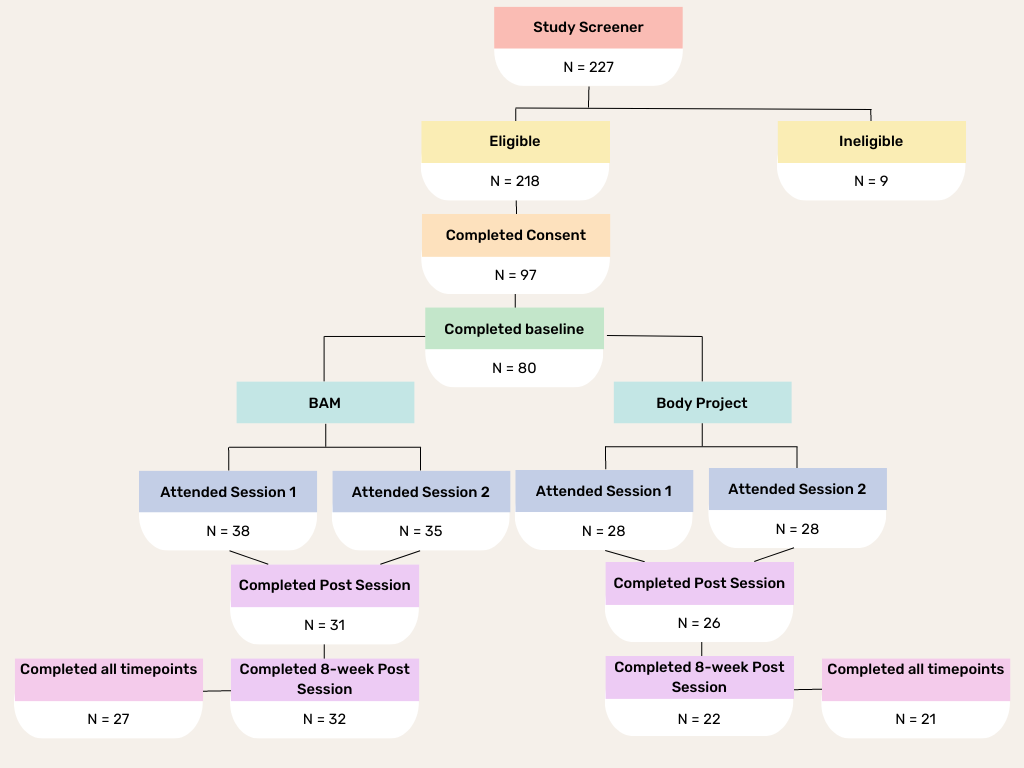
\includegraphics{./BAM_Study_Flow.png}

}

\caption{Figure 1: Study Flow Diagram}

\end{figure}

\bookmarksetup{startatroot}

\hypertarget{feasibility}{%
\chapter{Feasibility}\label{feasibility}}

To ensure peer facilitators presented the intervention scripts
accurately, all sessions were audio recorded and reviewed by two
research coordinators to assess for fidelity. Coordinators rated each
intervention section on a score of 0-10 based on how exact facilitators
presented the material.

\bookmarksetup{startatroot}

\hypertarget{acceptability}{%
\chapter{Acceptability}\label{acceptability}}

Analyses using a one-way analysis of variance (ANOVA) showed the two
groups did not significantly vary based on gender, race, or sexuality.
Attrition rate for the BAM intervention was 5\% with only 2 participants
dropping from the study between the first and second sessions, thus
confirming our hypothesis of the BAM intervention attrition being less
than 20\%. Zero participants dropped out of the Body Project group
between intervention sessions. Fifty participants (BAM: N = 26; Body
Project: N = 24) completed study activities at all three time points and
attended both intervention sessions.

Some participants were also asked to complete a feedback survey about
their experience with the BAM intervention at both the post session and
8-week post session time points.

\bookmarksetup{startatroot}

\hypertarget{intervention-effects}{%
\chapter{Intervention Effects}\label{intervention-effects}}

\hypertarget{fatphobia}{%
\section{Fatphobia}\label{fatphobia}}

Fatphobia was assessed at the three time points for both BAM (N = 26)
and Body Project (N = 24) participants using the Goldfarb Fear of Fat
Scale (\textbf{goldfarbGoldfarbFearFat1985?}).

Within the BAM group, the effect sizes for GFFS were as follows:

\begin{itemize}
\item
  The effect size between baseline and post-session was -0.51,
  indicating {[}interpretation of effect size{]}.
\item
  The effect size between baseline and 8 weeks was -0.35, indicating
  {[}interpretation of effect size{]}.
\item
  The effect size between post-session and 8 weeks was 0.16, indicating
  {[}interpretation of effect size{]}.
\end{itemize}

Within the Body Project group, the effect sizes for GFFS were as
follows:

\begin{itemize}
\item
  The effect size between baseline and post-session was -0.61,
  indicating {[}interpretation of effect size{]}.
\item
  The effect size between baseline and 8 weeks was -0.6, indicating
  {[}interpretation of effect size{]}.
\item
  The effect size between post-session and 8 weeks was 0.01, indicating
  {[}interpretation of effect size{]}.
\end{itemize}

\hypertarget{anti-fat-bias}{%
\section{Anti-fat Bias}\label{anti-fat-bias}}

Anti-fat Bias was also assessed at all three time points using the
Universal Measure of Bias-FAT
(UMB-FAT)(\textbf{dursoUnderstandingSelfdirectedStigma2008?}) and the
Eating Pathology Symptoms Inventory (EPSI) negative attitudes toward
obesity subcale (\textbf{coniglioFactorialIntegrityValidation2018?}).

Within the BAM group, the effect sizes for UMB-FAT were as follows:

\begin{itemize}
\item
  The effect size between baseline and post-session was -0.59,
  indicating {[}interpretation of effect size{]}.
\item
  The effect size between baseline and 8 weeks was -0.25, indicating
  {[}interpretation of effect size{]}.
\item
  The effect size between post-session and 8 weeks was 0.33, indicating
  {[}interpretation of effect size{]}.
\end{itemize}

Within the Body Project group, the effect sizes for UMB-FAT were as
follows:

\begin{itemize}
\item
  The effect size between baseline and post-session was -0.24,
  indicating {[}interpretation of effect size{]}.
\item
  The effect size between baseline and 8 weeks was -0.06, indicating
  {[}interpretation of effect size{]}.
\item
  The effect size between post-session and 8 weeks was 0.14, indicating
  {[}interpretation of effect size{]}.
\end{itemize}

\hypertarget{thin-ideal-internalization}{%
\section{Thin Ideal Internalization}\label{thin-ideal-internalization}}

Furthermore, thin ideal internalization was assessed using the
Sociocultural Attitudes Towards Appearance Questionnaire (SATAQ)
(\textbf{schaeferDevelopmentValidationSociocultural2015?}) and the Ideal
Body Stereotype Scale - Revised (IBSS-R)
(\textbf{sticeTestDualPathway1996?}).

Within the BAM group, the effect sizes for SATAQ were as follows:

\begin{itemize}
\item
  The effect size between baseline and post-session was -0.47,
  indicating {[}interpretation of effect size{]}.
\item
  The effect size between baseline and 8 weeks was -0.18, indicating
  {[}interpretation of effect size{]}.
\item
  The effect size between post-session and 8 weeks was 0.27, indicating
  {[}interpretation of effect size{]}.
\end{itemize}

Within the Body Project group, the effect sizes for SATAQ were as
follows:

\begin{itemize}
\item
  The effect size between baseline and post-session was -0.41,
  indicating {[}interpretation of effect size{]}.
\item
  The effect size between baseline and 8 weeks was -0.12, indicating
  {[}interpretation of effect size{]}.
\item
  The effect size between post-session and 8 weeks was 0.24, indicating
  {[}interpretation of effect size{]}.
\end{itemize}

Furthermore, the effect sizes for the IBSS-R for the BAM group were:

\begin{itemize}
\item
  The effect size between baseline and post-session was -0.82,
  indicating {[}interpretation of effect size{]}.
\item
  The effect size between baseline and 8 weeks was -0.47, indicating
  {[}interpretation of effect size{]}.
\item
  The effect size between post-session and 8 weeks was 0.2, indicating
  {[}interpretation of effect size{]}.
\end{itemize}

Within the Body Project group, the effect sizes for IBSS-R were as
follows:

\begin{itemize}
\item
  The effect size between baseline and post-session was -0.52,
  indicating {[}interpretation of effect size{]}.
\item
  The effect size between baseline and 8 weeks was -0.47, indicating
  {[}interpretation of effect size{]}.
\item
  The effect size between post-session and 8 weeks was 0.02, indicating
  {[}interpretation of effect size{]}.
\end{itemize}

\begin{longtable}[]{@{}
  >{\raggedright\arraybackslash}p{(\columnwidth - 10\tabcolsep) * \real{0.1667}}
  >{\raggedright\arraybackslash}p{(\columnwidth - 10\tabcolsep) * \real{0.1667}}
  >{\raggedright\arraybackslash}p{(\columnwidth - 10\tabcolsep) * \real{0.1667}}
  >{\raggedright\arraybackslash}p{(\columnwidth - 10\tabcolsep) * \real{0.1667}}
  >{\raggedright\arraybackslash}p{(\columnwidth - 10\tabcolsep) * \real{0.1667}}
  >{\raggedright\arraybackslash}p{(\columnwidth - 10\tabcolsep) * \real{0.1667}}@{}}
\toprule()
\begin{minipage}[b]{\linewidth}\raggedright
Measure
\end{minipage} & \begin{minipage}[b]{\linewidth}\raggedright
Variable
\end{minipage} & \begin{minipage}[b]{\linewidth}\raggedright
Group
\end{minipage} & \begin{minipage}[b]{\linewidth}\raggedright
Base to Post
\end{minipage} & \begin{minipage}[b]{\linewidth}\raggedright
Base to 8wk
\end{minipage} & \begin{minipage}[b]{\linewidth}\raggedright
Post to 8wk
\end{minipage} \\
\midrule()
\endhead
GFFS & gffs\_sum\_25 & BAM & -0.51 & -0.35 & 0.16 \\
& & Body Project & -0.61 & -0.6 & 0.01 \\
UMB-FAT & umb\_total\_sum & BAM & -0.59 & -0.25 & 0.33 \\
& & Body Project & -0.24 & -0.06 & 0.14 \\
SATAQ & sataq\_average & BAM & -0.47 & -0.18 & 0.27 \\
& & Body Project & -0.41 & -0.12 & 0.24 \\
IBSS-R & ibssr\_mean\_25 & BAM & -0.82 & -0.47 & 0.2 \\
& & Body Project & -0.52 & -0.47 & 0.02 \\
\bottomrule()
\end{longtable}

\bookmarksetup{startatroot}

\hypertarget{intervention-effects-ks}{%
\chapter{Intervention Effects KS}\label{intervention-effects-ks}}

\begin{Shaded}
\begin{Highlighting}[]
\NormalTok{mean\_list }\OtherTok{\textless{}{-}} \FunctionTok{list}\NormalTok{()}

\ControlFlowTok{for}\NormalTok{ (i }\ControlFlowTok{in}\NormalTok{ target\_vars) \{ }
\NormalTok{  mean\_df }\OtherTok{\textless{}{-}}\NormalTok{ BAM\_redcap\_long\_merged }\SpecialCharTok{\%\textgreater{}\%}
    \FunctionTok{filter}\NormalTok{(}\SpecialCharTok{!}\FunctionTok{is.na}\NormalTok{(timepoint), id }\SpecialCharTok{\%in\%}\NormalTok{ completers) }\SpecialCharTok{\%\textgreater{}\%}
    \FunctionTok{group\_by}\NormalTok{(timepoint, group) }\SpecialCharTok{\%\textgreater{}\%}
    \FunctionTok{summarise}\NormalTok{(}\AttributeTok{Mean =} \FunctionTok{mean}\NormalTok{(}\SpecialCharTok{!!}\FunctionTok{sym}\NormalTok{(i), }\AttributeTok{na.rm =} \ConstantTok{TRUE}\NormalTok{), }\AttributeTok{Variable =}\NormalTok{ i)  }\CommentTok{\# Use !!sym(i) to refer to the variable name dynamically}
    
\NormalTok{  mean\_list[[i]] }\OtherTok{\textless{}{-}}\NormalTok{ mean\_df}
\NormalTok{\}}
\end{Highlighting}
\end{Shaded}

\begin{verbatim}
`summarise()` has grouped output by 'timepoint'. You can override using the
`.groups` argument.
`summarise()` has grouped output by 'timepoint'. You can override using the
`.groups` argument.
`summarise()` has grouped output by 'timepoint'. You can override using the
`.groups` argument.
`summarise()` has grouped output by 'timepoint'. You can override using the
`.groups` argument.
`summarise()` has grouped output by 'timepoint'. You can override using the
`.groups` argument.
\end{verbatim}

\begin{Shaded}
\begin{Highlighting}[]
\CommentTok{\# Create a data frame with the results}
\NormalTok{mean\_df }\OtherTok{\textless{}{-}} \FunctionTok{do.call}\NormalTok{(rbind, mean\_list)}

\FunctionTok{save}\NormalTok{(mean\_df, }\AttributeTok{file =} \StringTok{\textquotesingle{}tabs/results\_tables.RData\textquotesingle{}}\NormalTok{)}
\end{Highlighting}
\end{Shaded}

\begin{Shaded}
\begin{Highlighting}[]
\CommentTok{\# Assuming you have the dataset BAM\_redcap\_long\_merged and target\_vars defined as before}

\CommentTok{\# Filter BAM\_redcap\_long\_merged to include only completers with all three timepoints}
\NormalTok{completers }\OtherTok{\textless{}{-}} \FunctionTok{unique}\NormalTok{(}\FunctionTok{with}\NormalTok{(BAM\_redcap\_long\_merged, id[}\FunctionTok{ave}\NormalTok{(timepoint, id, }\AttributeTok{FUN =} \ControlFlowTok{function}\NormalTok{(x) }\FunctionTok{length}\NormalTok{(}\FunctionTok{unique}\NormalTok{(x))) }\SpecialCharTok{==} \DecValTok{3}\NormalTok{]))}

\CommentTok{\# Function to calculate Cohen\textquotesingle{}s d effect size}
\NormalTok{calculate\_cohens\_d }\OtherTok{\textless{}{-}} \ControlFlowTok{function}\NormalTok{(mean1, mean2, sd\_pooled) \{}
\NormalTok{  mean\_diff }\OtherTok{\textless{}{-}}\NormalTok{ mean1 }\SpecialCharTok{{-}}\NormalTok{ mean2}
  \FunctionTok{return}\NormalTok{(mean\_diff }\SpecialCharTok{/}\NormalTok{ sd\_pooled)}
\NormalTok{\}}


\CommentTok{\# Function to calculate pooled standard deviation}
\NormalTok{pooled\_sd }\OtherTok{\textless{}{-}} \ControlFlowTok{function}\NormalTok{(n1, sd1, n2, sd2) \{}
  \FunctionTok{return}\NormalTok{(}\FunctionTok{sqrt}\NormalTok{(((n1 }\SpecialCharTok{{-}} \DecValTok{1}\NormalTok{) }\SpecialCharTok{*}\NormalTok{ sd1}\SpecialCharTok{\^{}}\DecValTok{2} \SpecialCharTok{+}\NormalTok{ (n2 }\SpecialCharTok{{-}} \DecValTok{1}\NormalTok{) }\SpecialCharTok{*}\NormalTok{ sd2}\SpecialCharTok{\^{}}\DecValTok{2}\NormalTok{) }\SpecialCharTok{/}\NormalTok{ (n1 }\SpecialCharTok{+}\NormalTok{ n2 }\SpecialCharTok{{-}} \DecValTok{2}\NormalTok{)))}
\NormalTok{\}}

\NormalTok{effect\_sizes\_list }\OtherTok{\textless{}{-}} \FunctionTok{list}\NormalTok{()}

\ControlFlowTok{for}\NormalTok{ (i }\ControlFlowTok{in}\NormalTok{ target\_vars) \{}
  \CommentTok{\# Filter the data for the current target variable and only completers}
\NormalTok{  filtered\_data }\OtherTok{\textless{}{-}}\NormalTok{ BAM\_redcap\_long\_merged }\SpecialCharTok{\%\textgreater{}\%}
    \FunctionTok{filter}\NormalTok{(id }\SpecialCharTok{\%in\%}\NormalTok{ completers) }\SpecialCharTok{\%\textgreater{}\%}
    \FunctionTok{select}\NormalTok{(group, timepoint, }\SpecialCharTok{!!}\FunctionTok{sym}\NormalTok{(i))}
  
  \CommentTok{\# Calculate the means and standard deviations for each timepoint within each group}
\NormalTok{  means\_sd }\OtherTok{\textless{}{-}}\NormalTok{ filtered\_data }\SpecialCharTok{\%\textgreater{}\%}
    \FunctionTok{group\_by}\NormalTok{(group, timepoint) }\SpecialCharTok{\%\textgreater{}\%}
    \FunctionTok{summarise}\NormalTok{(}
      \AttributeTok{Mean =} \FunctionTok{mean}\NormalTok{(}\SpecialCharTok{!!}\FunctionTok{sym}\NormalTok{(i), }\AttributeTok{na.rm =} \ConstantTok{TRUE}\NormalTok{),}
      \AttributeTok{SD =} \FunctionTok{sd}\NormalTok{(}\SpecialCharTok{!!}\FunctionTok{sym}\NormalTok{(i), }\AttributeTok{na.rm =} \ConstantTok{TRUE}\NormalTok{)}
\NormalTok{    )}
  
  \CommentTok{\# Extract the mean and standard deviation for each timepoint}
\NormalTok{  baseline\_mean }\OtherTok{\textless{}{-}}\NormalTok{ means\_sd }\SpecialCharTok{\%\textgreater{}\%}
    \FunctionTok{filter}\NormalTok{(timepoint }\SpecialCharTok{==} \StringTok{"baseline"}\NormalTok{) }\SpecialCharTok{\%\textgreater{}\%}
    \FunctionTok{pull}\NormalTok{(Mean)}
\NormalTok{  post\_mean }\OtherTok{\textless{}{-}}\NormalTok{ means\_sd }\SpecialCharTok{\%\textgreater{}\%}
    \FunctionTok{filter}\NormalTok{(timepoint }\SpecialCharTok{==} \StringTok{"post"}\NormalTok{) }\SpecialCharTok{\%\textgreater{}\%}
    \FunctionTok{pull}\NormalTok{(Mean)}
\NormalTok{  week8\_mean }\OtherTok{\textless{}{-}}\NormalTok{ means\_sd }\SpecialCharTok{\%\textgreater{}\%}
    \FunctionTok{filter}\NormalTok{(timepoint }\SpecialCharTok{==} \StringTok{"8wk"}\NormalTok{) }\SpecialCharTok{\%\textgreater{}\%}
    \FunctionTok{pull}\NormalTok{(Mean)}
  
\NormalTok{  baseline\_sd }\OtherTok{\textless{}{-}}\NormalTok{ means\_sd }\SpecialCharTok{\%\textgreater{}\%}
    \FunctionTok{filter}\NormalTok{(timepoint }\SpecialCharTok{==} \StringTok{"baseline"}\NormalTok{) }\SpecialCharTok{\%\textgreater{}\%}
    \FunctionTok{pull}\NormalTok{(SD)}
\NormalTok{  post\_sd }\OtherTok{\textless{}{-}}\NormalTok{ means\_sd }\SpecialCharTok{\%\textgreater{}\%}
    \FunctionTok{filter}\NormalTok{(timepoint }\SpecialCharTok{==} \StringTok{"post"}\NormalTok{) }\SpecialCharTok{\%\textgreater{}\%}
    \FunctionTok{pull}\NormalTok{(SD)}
\NormalTok{  week8\_sd }\OtherTok{\textless{}{-}}\NormalTok{ means\_sd }\SpecialCharTok{\%\textgreater{}\%}
    \FunctionTok{filter}\NormalTok{(timepoint }\SpecialCharTok{==} \StringTok{"8wk"}\NormalTok{) }\SpecialCharTok{\%\textgreater{}\%}
    \FunctionTok{pull}\NormalTok{(SD)}
  
  \CommentTok{\# Calculate Cohen\textquotesingle{}s d effect size for baseline{-}post and baseline{-}8wk comparisons within each group}
\NormalTok{  cohen\_d\_baseline\_post }\OtherTok{\textless{}{-}} \FunctionTok{calculate\_cohens\_d}\NormalTok{(post\_mean, baseline\_mean, }\FunctionTok{pooled\_sd}\NormalTok{(}\FunctionTok{nrow}\NormalTok{(filtered\_data }\SpecialCharTok{\%\textgreater{}\%} \FunctionTok{filter}\NormalTok{(timepoint }\SpecialCharTok{==} \StringTok{"post"}\NormalTok{)), post\_sd, }\FunctionTok{nrow}\NormalTok{(filtered\_data }\SpecialCharTok{\%\textgreater{}\%} \FunctionTok{filter}\NormalTok{(timepoint }\SpecialCharTok{==} \StringTok{"baseline"}\NormalTok{)), baseline\_sd))}
\NormalTok{  cohen\_d\_baseline\_8\_week }\OtherTok{\textless{}{-}} \FunctionTok{calculate\_cohens\_d}\NormalTok{(week8\_mean, baseline\_mean, }\FunctionTok{pooled\_sd}\NormalTok{(}\FunctionTok{nrow}\NormalTok{(filtered\_data }\SpecialCharTok{\%\textgreater{}\%} \FunctionTok{filter}\NormalTok{(timepoint }\SpecialCharTok{==} \StringTok{"8wk"}\NormalTok{)), week8\_sd, }\FunctionTok{nrow}\NormalTok{(filtered\_data }\SpecialCharTok{\%\textgreater{}\%} \FunctionTok{filter}\NormalTok{(timepoint }\SpecialCharTok{==} \StringTok{"baseline"}\NormalTok{)), baseline\_sd))}
  
  \CommentTok{\# Create a data frame to store the effect sizes for the current target variable}
\NormalTok{  result }\OtherTok{\textless{}{-}} \FunctionTok{data.frame}\NormalTok{(}
    \AttributeTok{group =} \FunctionTok{unique}\NormalTok{(filtered\_data}\SpecialCharTok{$}\NormalTok{group),}
    \AttributeTok{Variable =}\NormalTok{ i,}
    \AttributeTok{Cohens\_d\_baseline\_post =}\NormalTok{ cohen\_d\_baseline\_post,}
    \AttributeTok{Cohens\_d\_baseline\_8\_week =}\NormalTok{ cohen\_d\_baseline\_8\_week}
\NormalTok{  )}
  
\NormalTok{  effect\_sizes\_list[[i]] }\OtherTok{\textless{}{-}}\NormalTok{ result}
\NormalTok{\}}
\end{Highlighting}
\end{Shaded}

\begin{verbatim}
`summarise()` has grouped output by 'group'. You can override using the
`.groups` argument.
`summarise()` has grouped output by 'group'. You can override using the
`.groups` argument.
`summarise()` has grouped output by 'group'. You can override using the
`.groups` argument.
`summarise()` has grouped output by 'group'. You can override using the
`.groups` argument.
`summarise()` has grouped output by 'group'. You can override using the
`.groups` argument.
\end{verbatim}

\begin{Shaded}
\begin{Highlighting}[]
\CommentTok{\# Combine all effect sizes for different target variables into a single data frame}
\NormalTok{effect\_sizes\_df }\OtherTok{\textless{}{-}} \FunctionTok{do.call}\NormalTok{(rbind, effect\_sizes\_list)}

\FunctionTok{resave}\NormalTok{(effect\_sizes\_df, }\AttributeTok{file =} \StringTok{\textquotesingle{}tabs/results\_tables.RData\textquotesingle{}}\NormalTok{)}
\end{Highlighting}
\end{Shaded}

\begin{Shaded}
\begin{Highlighting}[]
\FunctionTok{rm}\NormalTok{(}\AttributeTok{list =} \FunctionTok{ls}\NormalTok{()[}\SpecialCharTok{!}\FunctionTok{ls}\NormalTok{() }\SpecialCharTok{\%in\%} \FunctionTok{c}\NormalTok{(}\StringTok{"BAM\_redcap\_long\_merged"}\NormalTok{, }\StringTok{"mean\_df"}\NormalTok{, }\StringTok{"effect\_sizes\_df"}\NormalTok{, }\StringTok{\textquotesingle{}completers\textquotesingle{}}\NormalTok{, }\StringTok{\textquotesingle{}target\_vars\textquotesingle{}}\NormalTok{)])}
\end{Highlighting}
\end{Shaded}

\begin{Shaded}
\begin{Highlighting}[]
\CommentTok{\# Function to calculate standard error}
\NormalTok{standard\_error }\OtherTok{\textless{}{-}} \ControlFlowTok{function}\NormalTok{(x) \{}
  \FunctionTok{return}\NormalTok{(}\FunctionTok{sd}\NormalTok{(x, }\AttributeTok{na.rm =} \ConstantTok{TRUE}\NormalTok{) }\SpecialCharTok{/} \FunctionTok{sqrt}\NormalTok{(}\FunctionTok{length}\NormalTok{(x)))}
\NormalTok{\}}

\CommentTok{\# Create a list to store the ggplot objects}
\NormalTok{ggplot\_list }\OtherTok{\textless{}{-}} \FunctionTok{list}\NormalTok{()}

\ControlFlowTok{for}\NormalTok{ (i }\ControlFlowTok{in}\NormalTok{ target\_vars) \{}
  \CommentTok{\# Filter the data for the current target variable and only completers}
\NormalTok{  filtered\_data }\OtherTok{\textless{}{-}}\NormalTok{ BAM\_redcap\_long\_merged }\SpecialCharTok{\%\textgreater{}\%}
    \FunctionTok{filter}\NormalTok{(id }\SpecialCharTok{\%in\%}\NormalTok{ completers) }\SpecialCharTok{\%\textgreater{}\%}
    \FunctionTok{select}\NormalTok{(group, timepoint, }\SpecialCharTok{!!}\FunctionTok{sym}\NormalTok{(i))}

  
\NormalTok{    filtered\_data}\SpecialCharTok{$}\NormalTok{timepoint }\OtherTok{\textless{}{-}} \FunctionTok{factor}\NormalTok{(filtered\_data}\SpecialCharTok{$}\NormalTok{timepoint, }\AttributeTok{levels =} \FunctionTok{c}\NormalTok{(}\StringTok{"baseline"}\NormalTok{, }\StringTok{"post"}\NormalTok{, }\StringTok{"8wk"}\NormalTok{))}
    
  \CommentTok{\# Calculate the means and standard errors for each timepoint within each group}
\NormalTok{  means\_se }\OtherTok{\textless{}{-}}\NormalTok{ filtered\_data }\SpecialCharTok{\%\textgreater{}\%}
    \FunctionTok{group\_by}\NormalTok{(group, timepoint) }\SpecialCharTok{\%\textgreater{}\%}
    \FunctionTok{summarise}\NormalTok{(}
      \AttributeTok{Mean =} \FunctionTok{mean}\NormalTok{(}\SpecialCharTok{!!}\FunctionTok{sym}\NormalTok{(i), }\AttributeTok{na.rm =} \ConstantTok{TRUE}\NormalTok{),}
      \AttributeTok{SE =} \FunctionTok{standard\_error}\NormalTok{(}\SpecialCharTok{!!}\FunctionTok{sym}\NormalTok{(i))}
\NormalTok{    )}
  
  \CommentTok{\# Plot the line graph with separate lines for each group}
\NormalTok{  p }\OtherTok{\textless{}{-}} \FunctionTok{ggplot}\NormalTok{(means\_se, }\FunctionTok{aes}\NormalTok{(}\AttributeTok{x =}\NormalTok{ timepoint, }\AttributeTok{y =}\NormalTok{ Mean, }\AttributeTok{group =}\NormalTok{ group, }\AttributeTok{color =}\NormalTok{ group)) }\SpecialCharTok{+}
    \FunctionTok{geom\_line}\NormalTok{() }\SpecialCharTok{+}
    \FunctionTok{geom\_point}\NormalTok{() }\SpecialCharTok{+}
    \FunctionTok{geom\_errorbar}\NormalTok{(}\FunctionTok{aes}\NormalTok{(}\AttributeTok{ymin =}\NormalTok{ Mean }\SpecialCharTok{{-}}\NormalTok{ SE, }\AttributeTok{ymax =}\NormalTok{ Mean }\SpecialCharTok{+}\NormalTok{ SE), }\AttributeTok{width =} \FloatTok{0.1}\NormalTok{) }\SpecialCharTok{+}
    \FunctionTok{labs}\NormalTok{(}\AttributeTok{title =} \FunctionTok{paste}\NormalTok{(i), }\AttributeTok{x =} \StringTok{"Timepoint"}\NormalTok{, }\AttributeTok{y =} \StringTok{"Mean"}\NormalTok{, }\AttributeTok{color =} \StringTok{"Group"}\NormalTok{) }\SpecialCharTok{+}
    \FunctionTok{theme\_minimal}\NormalTok{()}
  
\NormalTok{  ggplot\_list[[i]] }\OtherTok{\textless{}{-}}\NormalTok{ p}
\NormalTok{\}}
\end{Highlighting}
\end{Shaded}

\begin{verbatim}
`summarise()` has grouped output by 'group'. You can override using the
`.groups` argument.
`summarise()` has grouped output by 'group'. You can override using the
`.groups` argument.
`summarise()` has grouped output by 'group'. You can override using the
`.groups` argument.
`summarise()` has grouped output by 'group'. You can override using the
`.groups` argument.
`summarise()` has grouped output by 'group'. You can override using the
`.groups` argument.
\end{verbatim}

\begin{Shaded}
\begin{Highlighting}[]
\NormalTok{combined\_plots }\OtherTok{\textless{}{-}}\NormalTok{ ggplot\_list[[}\DecValTok{1}\NormalTok{]] }\SpecialCharTok{+} \FunctionTok{plot\_layout}\NormalTok{(}\AttributeTok{ncol =} \DecValTok{2}\NormalTok{)}
\ControlFlowTok{for}\NormalTok{ (i }\ControlFlowTok{in} \DecValTok{2}\SpecialCharTok{:}\FunctionTok{length}\NormalTok{(target\_vars)) \{}
\NormalTok{  combined\_plots }\OtherTok{\textless{}{-}}\NormalTok{ combined\_plots }\SpecialCharTok{+}\NormalTok{ ggplot\_list[[i]]}
\NormalTok{\}}

\NormalTok{combined\_plots}
\end{Highlighting}
\end{Shaded}

\begin{figure}[H]

{\centering 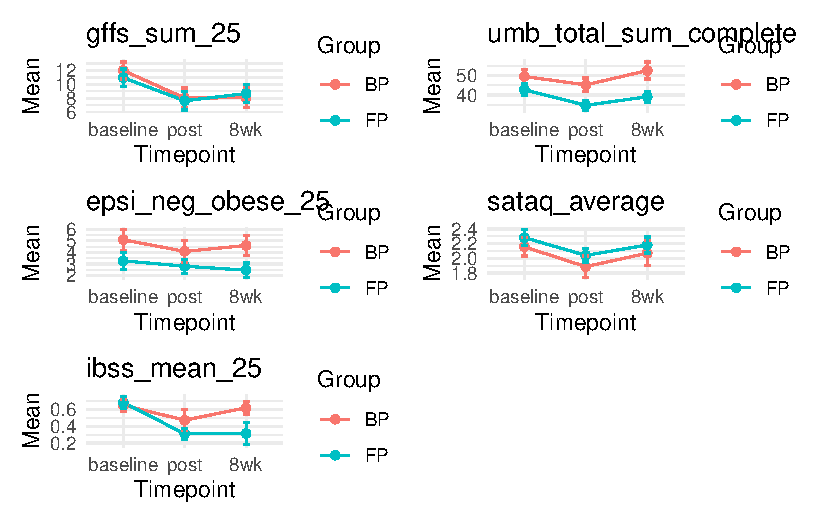
\includegraphics{./InterventionEffects.KS_files/figure-pdf/unnamed-chunk-5-1.pdf}

}

\end{figure}

\begin{Shaded}
\begin{Highlighting}[]
\FunctionTok{ggsave}\NormalTok{(}\AttributeTok{plot =}\NormalTok{ combined\_plots, }\AttributeTok{file =} \StringTok{\textquotesingle{}figs/targets.png\textquotesingle{}}\NormalTok{)}
\end{Highlighting}
\end{Shaded}

\begin{verbatim}
Saving 5.5 x 3.5 in image
\end{verbatim}

\begin{Shaded}
\begin{Highlighting}[]
\FunctionTok{library}\NormalTok{(knitr)}
\FunctionTok{load}\NormalTok{(}\StringTok{"tabs/results\_tables.RData"}\NormalTok{)}
\NormalTok{knitr}\SpecialCharTok{::}\FunctionTok{kable}\NormalTok{(effect\_sizes\_df, }\AttributeTok{format =} \StringTok{"html"}\NormalTok{, }\AttributeTok{caption =} \StringTok{"Effect Sizes Table"}\NormalTok{)}
\end{Highlighting}
\end{Shaded}

\begin{longtable}[]{@{}lllrr@{}}
\caption{Effect Sizes Table}\tabularnewline
\toprule()
& group & Variable & Cohens\_d\_baseline\_post &
Cohens\_d\_baseline\_8\_week \\
\midrule()
\endfirsthead
\toprule()
& group & Variable & Cohens\_d\_baseline\_post &
Cohens\_d\_baseline\_8\_week \\
\midrule()
\endhead
gffs\_sum\_25.1 & BP & gffs\_sum\_25 & -0.6084333 & -0.5972547 \\
gffs\_sum\_25.2 & FP & gffs\_sum\_25 & -0.5050240 & -0.3524653 \\
umb\_total\_sum\_complete.1 & BP & umb\_total\_sum\_complete &
-0.2426019 & 0.1516238 \\
umb\_total\_sum\_complete.2 & FP & umb\_total\_sum\_complete &
-0.5949443 & -0.2453964 \\
epsi\_neg\_obese\_25.1 & BP & epsi\_neg\_obese\_25 & -0.2243805 &
-0.1158431 \\
epsi\_neg\_obese\_25.2 & FP & epsi\_neg\_obese\_25 & -0.1328859 &
-0.2309433 \\
sataq\_average.1 & BP & sataq\_average & -0.4062737 & -0.1186174 \\
sataq\_average.2 & FP & sataq\_average & -0.4668367 & -0.1792651 \\
ibss\_mean\_25.1 & BP & ibss\_mean\_25 & -0.3524714 & -0.0872552 \\
ibss\_mean\_25.2 & FP & ibss\_mean\_25 & -1.1116491 & -0.6813379 \\
\bottomrule()
\end{longtable}

\begin{Shaded}
\begin{Highlighting}[]
\NormalTok{knitr}\SpecialCharTok{::}\FunctionTok{kable}\NormalTok{(mean\_df, }\AttributeTok{format =} \StringTok{"html"}\NormalTok{, }\AttributeTok{caption =} \StringTok{"Mean Table"}\NormalTok{)}
\end{Highlighting}
\end{Shaded}

\begin{longtable}[]{@{}llrl@{}}
\caption{Mean Table}\tabularnewline
\toprule()
timepoint & group & Mean & Variable \\
\midrule()
\endfirsthead
\toprule()
timepoint & group & Mean & Variable \\
\midrule()
\endhead
8wk & BP & 8.0909091 & gffs\_sum\_25 \\
8wk & FP & 8.6923077 & gffs\_sum\_25 \\
baseline & BP & 12.0000000 & gffs\_sum\_25 \\
baseline & FP & 10.9615385 & gffs\_sum\_25 \\
post & BP & 8.0416667 & gffs\_sum\_25 \\
post & FP & 7.6538462 & gffs\_sum\_25 \\
8wk & BP & 52.6363636 & umb\_total\_sum\_complete \\
8wk & FP & 39.0769231 & umb\_total\_sum\_complete \\
baseline & BP & 49.5833333 & umb\_total\_sum\_complete \\
baseline & FP & 42.7307692 & umb\_total\_sum\_complete \\
post & BP & 45.2083333 & umb\_total\_sum\_complete \\
post & FP & 34.6153846 & umb\_total\_sum\_complete \\
8wk & BP & 4.5909091 & epsi\_neg\_obese\_25 \\
8wk & FP & 2.4615385 & epsi\_neg\_obese\_25 \\
baseline & BP & 5.0833333 & epsi\_neg\_obese\_25 \\
baseline & FP & 3.2692308 & epsi\_neg\_obese\_25 \\
post & BP & 4.0833333 & epsi\_neg\_obese\_25 \\
post & FP & 2.8076923 & epsi\_neg\_obese\_25 \\
8wk & BP & 2.0702479 & sataq\_average \\
8wk & FP & 2.1818182 & sataq\_average \\
baseline & BP & 2.1571970 & sataq\_average \\
baseline & FP & 2.2832168 & sataq\_average \\
post & BP & 1.8863636 & sataq\_average \\
post & FP & 2.0402098 & sataq\_average \\
8wk & BP & 0.6208333 & ibss\_mean\_25 \\
8wk & FP & 0.3142857 & ibss\_mean\_25 \\
baseline & BP & 0.6518519 & ibss\_mean\_25 \\
baseline & FP & 0.6833333 & ibss\_mean\_25 \\
post & BP & 0.4733333 & ibss\_mean\_25 \\
post & FP & 0.3111111 & ibss\_mean\_25 \\
\bottomrule()
\end{longtable}

\bookmarksetup{startatroot}

\hypertarget{references}{%
\chapter*{References}\label{references}}
\addcontentsline{toc}{chapter}{References}

\hypertarget{refs}{}
\begin{CSLReferences}{0}{0}
\end{CSLReferences}



\end{document}
